A sample accessibility plug-in for certain elements of the Logic Diagram sample plug-in project (contributed from the GEF plug-ins to Eclipse's New Project Wizard) are included in the installation of \jb{}. You can import the sample accessibility plug-in into an Eclipse workspace in order to examine the general structure of such an accessibility plug-in (\bxfigref{newlogicwizard})

\begin{figure}[h]
\begin{center}
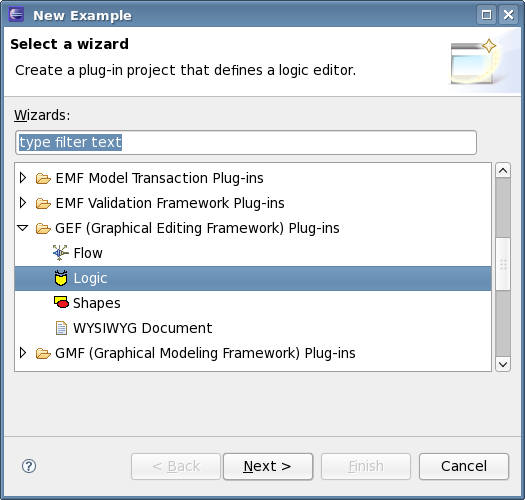
\includegraphics[width=12.5cm]{Tasks/GEF/PS/newlogicwizard}
\caption{Creating the 'Logic' Project}
\label{newlogicwizard}
\end{center}
\end{figure}



The javadocs containing information about \bxname{com.bredexsw.guidancer.gef.identifier.IEditPartIdentifier} and default implementations can be found in the \jb{} installation directory under \bxname{documentation/gefapi/javadoc.zip}.
\clearpage
